% Simple Beamer Example
% SUZA LaTeX & AI Workshop - Day 2
% A clean template for creating academic presentations

\documentclass[aspectratio=169]{beamer}

% Choose your theme and color scheme
\usetheme{Madrid}
\usecolortheme{default}

% Packages
\usepackage[utf8]{inputenc}
\usepackage{graphicx}
\usepackage{amsmath}
\usepackage{booktabs}
\usepackage{hyperref}
\usepackage{tikz}
\usetikzlibrary{positioning,shapes,arrows}

% Title Information
\title{Your Research Title Here}
\subtitle{A Clear and Concise Subtitle}
\author{Your Name\\[0.2cm]
	{\small Supervisor: Dr. Supervisor Name}}
\institute{Department of Computer Science \& IT\\
	State University of Zanzibar}
\date{\today}

% Optional: Add logo
% \logo{\includegraphics[height=1cm]{../resources/suza_logo.png}}

% Remove navigation symbols (optional)
\setbeamertemplate{navigation symbols}{}

%==============================================================================
\begin{document}
	
	% Title Slide
	\begin{frame}
		\titlepage
	\end{frame}
	
	% Table of Contents
	\begin{frame}{Outline}
		\tableofcontents
	\end{frame}
	
	%==============================================================================
	\section{Introduction}
	
	\begin{frame}{Introduction}
		\begin{block}{Research Problem}
			State your research problem clearly and concisely.
		\end{block}
		
		\vspace{1em}
		
		\textbf{Key Points:}
		\begin{itemize}
			\item First important point
			\item Second important point
			\item Third important point
		\end{itemize}
	\end{frame}
	
	\begin{frame}{Background and Motivation}
		\begin{columns}
			\begin{column}{0.48\textwidth}
				\textbf{Why This Matters:}
				\begin{itemize}
					\item Reason 1
					\item Reason 2
					\item Reason 3
				\end{itemize}
			\end{column}
			
			\begin{column}{0.48\textwidth}
				\centering
				\fbox{\parbox{0.9\textwidth}{\centering\vspace{1.5cm}
						[Image Placeholder]
						\vspace{1.5cm}}}
			\end{column}
		\end{columns}
	\end{frame}
	
	\begin{frame}{Research Objectives}
		\begin{enumerate}
			\item<1-> \textbf{Primary Objective:} Main goal of the research
			\item<2-> \textbf{Specific Objective 1:} First detailed objective
			\item<3-> \textbf{Specific Objective 2:} Second detailed objective
			\item<4-> \textbf{Specific Objective 3:} Third detailed objective
		\end{enumerate}
		
		\vspace{1em}
		
		\uncover<5->{
			\begin{alertblock}{Note}
				These objectives build progressively on each other.
			\end{alertblock}
		}
	\end{frame}
	
	%==============================================================================
	\section{Literature Review}
	
	\begin{frame}{Key Concepts}
		\begin{definition}
			\textbf{Important Term:} Definition of the term that's central to your research.
		\end{definition}
		
		\vspace{1em}
		
		\begin{exampleblock}{Example}
			A practical example that illustrates the concept.
		\end{exampleblock}
	\end{frame}
	
	\begin{frame}{Related Work}
		\begin{table}
			\centering
			\caption{Summary of Related Studies}
			\begin{tabular}{lll}
				\toprule
				\textbf{Study} & \textbf{Method} & \textbf{Findings} \\
				\midrule
				Smith (2023) & Survey & Key finding \\
				Jones (2022) & Experiment & Key finding \\
				Brown (2021) & Analysis & Key finding \\
				\bottomrule
			\end{tabular}
		\end{table}
	\end{frame}
	
	\begin{frame}{Research Gap}
		\begin{alertblock}{The Gap}
			Despite previous research, there remains a gap in...
		\end{alertblock}
		
		\vspace{1em}
		
		\textbf{Our Contribution:}
		\begin{itemize}
			\item Novel approach or perspective
			\item New data or methodology
			\item Practical application
		\end{itemize}
	\end{frame}
	
	%==============================================================================
	\section{Methodology}
	
	\begin{frame}{Research Design}
		\begin{center}
			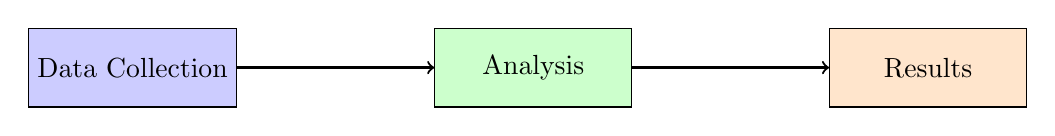
\begin{tikzpicture}[
				node distance=2.5cm,
				box/.style={rectangle, draw, fill=blue!20, minimum width=2.5cm, minimum height=1cm}
				]
				\node[box] (start) {Data Collection};
				\node[box, right=of start, fill=green!20] (process) {Analysis};
				\node[box, right=of process, fill=orange!20] (result) {Results};
				
				\draw[->, thick] (start) -- (process);
				\draw[->, thick] (process) -- (result);
			\end{tikzpicture}
		\end{center}
		
		\vspace{1em}
		
		\textbf{Approach:} Quantitative/Qualitative/Mixed Methods
	\end{frame}
	
	\begin{frame}{Data Collection}
		\textbf{Sample:}
		\begin{itemize}
			\item Population: Who/what was studied
			\item Sample size: $n = 150$ participants
			\item Sampling method: Random/Stratified/Convenience
		\end{itemize}
		
		\vspace{1em}
		
		\textbf{Instruments:}
		\begin{itemize}
			\item Questionnaires
			\item Interviews
			\item Observations
		\end{itemize}
	\end{frame}
	
	\begin{frame}{Analysis Methods}
		\textbf{Mathematical Model:}
		
		\begin{equation}
			y = \beta_0 + \beta_1 x_1 + \beta_2 x_2 + \epsilon
		\end{equation}
		
		where $y$ is the dependent variable, $x_i$ are predictors, $\beta_i$ are coefficients, and $\epsilon$ is the error term.
		
		\vspace{1em}
		
		\textbf{Software Used:}
		\begin{itemize}
			\item Python/R for statistical analysis
			\item SPSS/Excel for data management
		\end{itemize}
	\end{frame}
	
	%==============================================================================
	\section{Results}
	
	\begin{frame}{Key Findings}
		\begin{block}{Finding 1}
			Description of your first major finding.
		\end{block}
		
		\begin{block}{Finding 2}
			Description of your second major finding.
		\end{block}
		
		\begin{block}{Finding 3}
			Description of your third major finding.
		\end{block}
	\end{frame}
	
	\begin{frame}{Quantitative Results}
		\begin{columns}
			\begin{column}{0.48\textwidth}
				\begin{table}
					\centering
					\scriptsize
					\begin{tabular}{lc}
						\toprule
						\textbf{Metric} & \textbf{Value} \\
						\midrule
						Accuracy & 94.3\% \\
						Precision & 91.7\% \\
						Recall & 89.2\% \\
						F1-Score & 90.4\% \\
						\bottomrule
					\end{tabular}
				\end{table}
			\end{column}
			
			\begin{column}{0.48\textwidth}
				\centering
				\fbox{\parbox{0.9\textwidth}{\centering\vspace{2cm}
						[Chart/Graph]
						\vspace{2cm}}}
			\end{column}
		\end{columns}
	\end{frame}
	
	\begin{frame}{Visual Results}
		\begin{figure}
			\centering
			\fbox{\parbox{0.7\textwidth}{\centering\vspace{3cm}
					[Your Main Result Visualization]\\
					\vspace{0.5cm}
					This could be a chart, graph, diagram, or image
					\vspace{3cm}}}
			\caption{Caption describing the visualization}
		\end{figure}
	\end{frame}
	
	\begin{frame}{Statistical Significance}
		\textbf{Hypothesis Testing Results:}
		
		\begin{itemize}
			\item $H_0$: Null hypothesis statement
			\item $H_1$: Alternative hypothesis statement
			\item Test statistic: $t = 4.56$
			\item $p$-value: $p < 0.001$
			\item \textbf{Conclusion:} Reject $H_0$ at $\alpha = 0.05$ level
		\end{itemize}
		
		\vspace{1em}
		
		\begin{alertblock}{Interpretation}
			The results are statistically significant and support the alternative hypothesis.
		\end{alertblock}
	\end{frame}
	
	%==============================================================================
	\section{Discussion}
	
	\begin{frame}{Interpretation}
		\textbf{What do these results mean?}
		
		\begin{itemize}
			\item Connect back to research objectives
			\item Compare with previous studies
			\item Explain unexpected findings
			\item Discuss practical implications
		\end{itemize}
		
		\vspace{1em}
		
		\begin{exampleblock}{Key Insight}
			The most important takeaway from your research.
		\end{exampleblock}
	\end{frame}
	
	\begin{frame}{Limitations}
		\textbf{Limitations of this study:}
		
		\begin{enumerate}
			\item Sample size constraints
			\item Time limitations
			\item Scope of the study
			\item Data availability issues
		\end{enumerate}
		
		\vspace{1em}
		
		\textit{Being transparent about limitations strengthens your research credibility.}
	\end{frame}
	
	\begin{frame}{Future Work}
		\textbf{Directions for future research:}
		
		\begin{itemize}
			\item Expand the study to larger populations
			\item Investigate additional variables
			\item Apply findings in different contexts
			\item Develop practical applications
		\end{itemize}
		
		\vspace{1em}
		
		\textbf{Next Steps:}
		\begin{itemize}
			\item Immediate actions
			\item Long-term goals
		\end{itemize}
	\end{frame}
	
	%==============================================================================
	\section{Conclusion}
	
	\begin{frame}{Summary}
		\textbf{What we did:}
		\begin{itemize}
			\item Brief recap of methodology
		\end{itemize}
		
		\vspace{0.5em}
		
		\textbf{What we found:}
		\begin{itemize}
			\item Summary of key findings
		\end{itemize}
		
		\vspace{0.5em}
		
		\textbf{What it means:}
		\begin{itemize}
			\item Implications and significance
		\end{itemize}
	\end{frame}
	
	\begin{frame}{Main Conclusions}
		\begin{enumerate}
			\item \textbf{First major conclusion}
			\item \textbf{Second major conclusion}
			\item \textbf{Third major conclusion}
		\end{enumerate}
		
		\vspace{2em}
		
		\begin{center}
			\Large
			\textbf{Take-home message:}\\[0.5em]
			One sentence that captures the essence of your research.
		\end{center}
	\end{frame}
	
	\begin{frame}{Recommendations}
		\textbf{For Practitioners:}
		\begin{itemize}
			\item Practical recommendation 1
			\item Practical recommendation 2
		\end{itemize}
		
		\vspace{1em}
		
		\textbf{For Policy Makers:}
		\begin{itemize}
			\item Policy recommendation 1
			\item Policy recommendation 2
		\end{itemize}
		
		\vspace{1em}
		
		\textbf{For Researchers:}
		\begin{itemize}
			\item Research recommendation 1
			\item Research recommendation 2
		\end{itemize}
	\end{frame}
	
	%==============================================================================
	\section*{References}
	
	\begin{frame}[allowframebreaks]{References}
		\scriptsize
		\begin{thebibliography}{99}
			
			\bibitem{ref1}
			Smith, J. and Brown, A. (2023).
			\textit{Title of the Paper}.
			Journal Name, 45(2), 123-145.
			
			\bibitem{ref2}
			Jones, M. (2022).
			\textit{Book Title}.
			Publisher Name.
			
			\bibitem{ref3}
			Wilson, P. et al. (2021).
			Conference paper title.
			\textit{Proceedings of Conference Name}, pp. 567-578.
			
		\end{thebibliography}
	\end{frame}
	
	%==============================================================================
	\begin{frame}[plain]
		\centering
		\vspace{2em}
		
		{\Huge\textbf{Thank You!}}
		
		\vspace{2em}
		
		{\Large Questions?}
		
		\vspace{2em}
		
		{\normalsize
			Your Name\\
			your.email@suza.ac.tz\\
			Department of CS\&IT, SUZA}
	\end{frame}
	
	%==============================================================================
	% BACKUP SLIDES (Optional - not counted in main presentation time)
	%==============================================================================
	
	\appendix
	
	\begin{frame}{Additional Data}
		\begin{center}
			\textit{Backup slides for questions}
		\end{center}
		
		Additional tables, figures, or technical details that you might need to answer questions but don't fit in the main presentation.
	\end{frame}
	
	\begin{frame}{Detailed Methodology}
		More technical details about your methodology that might be asked about during Q\&A.
	\end{frame}
	
\end{document}